
\documentclass[xcolor=dvipsnames]{beamer}

\usetheme{Madrid}
\useoutertheme{miniframes} % Alternatively: miniframes, infolines, split
\useinnertheme{circles}
\usepackage{booktabs}
\newcommand{\ra}[1]{\renewcommand{\arraystretch}{#1}}

\definecolor{UBCblue}{rgb}{0.04706, 0.13725, 0.26667} % UBC Blue (primary)
\definecolor{UBCgrey}{rgb}{0.0, 0.87, 0.75} % Hatsune Miku Palette (secondary) NEON 
%\definecolor{UBCgrey}{rgb}{0.0, 0.6, 0.6} % Hatsune Miku Palette (secondary)  
%\definecolor{UBCgrey}{rgb}{0.3686, 0.5255, 0.6235} % cool neon feel w UBC blue 
%\definecolor{UBCblue}{rgb}{0.04706, 0.13725, 0.26667} % UBC Blue (primary)
%\definecolor{UBCgrey}{rgb}{0.3686, 0.999, 0.6235} % UBC Grey (secondary)

\setbeamercolor{palette primary}{bg=UBCblue,fg=white}
\setbeamercolor{palette secondary}{bg=UBCblue,fg=white}
\setbeamercolor{palette tertiary}{bg=UBCblue,fg=white}
\setbeamercolor{palette quaternary}{bg=UBCblue,fg=white}
\setbeamercolor{structure}{fg=UBCblue} % itemize, enumerate, etc
\setbeamercolor{section in toc}{fg=UBCblue} % TOC sections

% Override palette coloring with secondary
\setbeamercolor{subsection in head/foot}{bg=UBCgrey,fg=white}

\title[Meeting 2]{Enumeration and visualization of various subspaces of the octahedral complex space}
\date{April 27, 2018}
\author[Stefan O. Gugler]
{Stefan O. Gugler}
\institute[MIT]{Massachusetts Institute of Technology  \\Department of Chemical Engineering}

\begin{document}
	
\begin{frame}
	\titlepage
\end{frame}
%
%\begin{frame}
%	\tableofcontents
%\end{frame}

%% % % % % % % % % % % % % % % % %
%\section{Spaces and Properties}
%% % % % % % % % % % % % % % % % %
%\subsection{First Subsection}

\begin{frame}
\frametitle{Subsets of octahedral space}
The sizes of the selected subsets of octahedral space.
\begin{table}[]
	\centering
%	\caption{The sizes of the selected subsets of octahedral space.}
	\label{tab:space-sizes}
	\begin{tabular}{llr}
		\toprule
		Set 					& description		    	   & size \\
		\midrule
		Homoleptics             & eq = ax                   & 553        \\[0.1cm]
		"5+1" symmetric         & eq = ax1 $\neq$ ax2       & 163,620    \\[0.1cm]
		"4+2" symmetric         & eq1 $\neq$ eq2 = ax       & 185,373    \\[0.1cm]
		Strongly symmetric      & eq $\neq$ ax              & 245,316    \\[0.1cm]
		Equatorially asymmetric & eq1 $\neq$ eq2 $\neq$ ax  & 15,924,796 \\[0.1cm]
		Weakly symmetric        & eq $\neq$ ax1 $\neq$ ax2  & 45,077,310 \\[0.1cm]
		Complete Heteroleptics  & $L_i \neq L_j$            & $\approx 5.9 \cdot 10^{12}$ \\[0.1cm] %405!/399!/6!+148!/145!/3!
		Octahedral Space        & all                       & $> 1.8 \cdot 10^{14}$ \\
		%number of cube colorings as lower bound
		\bottomrule
	\end{tabular}
	\end{table}
\end{frame}


\begin{frame}
\frametitle{Properties of the sets}
\begin{itemize}
\item Reduce space to facilitate sampling from non-homoleptics
\item Example: strongly symmetric, monodentate ligand fields (163,620)
\item Exclude all with charge smaller than -4, which results in 87,150 ligand fields (53~\%).
\end{itemize}

\begin{figure}[ht] 
	\begin{minipage}[b]{0.5\linewidth}
		\centering
		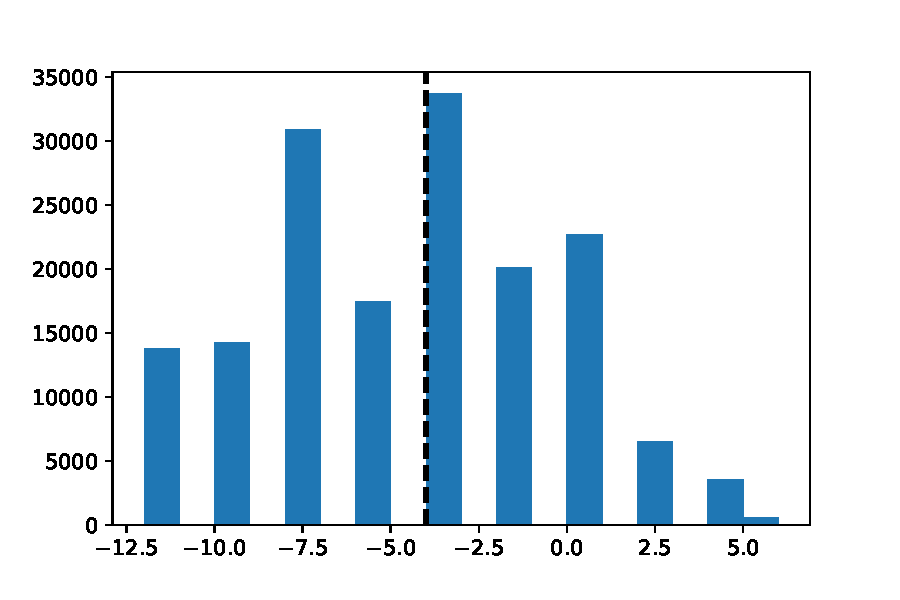
\includegraphics[width=.8\linewidth]{img/strongsymMonodentates_chargeHist.pdf} 
		\vspace{4ex}
	\end{minipage}%%
	\begin{minipage}[b]{0.5\linewidth}
		\centering
		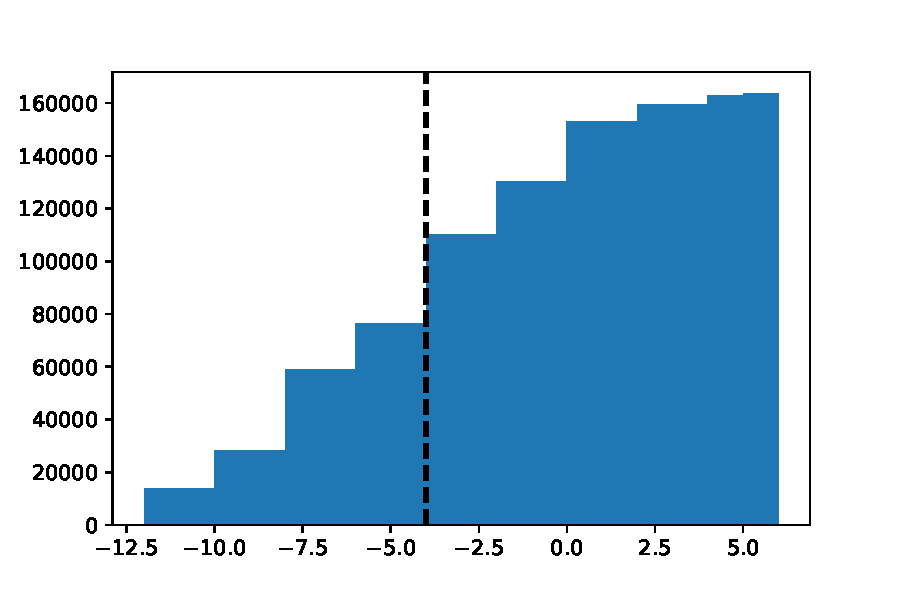
\includegraphics[width=.8\linewidth]{img/strongsymMonodentates_chargeHistCum.pdf} 
		\vspace{4ex}
	\end{minipage} 
\end{figure}
\end{frame}


\begin{frame}
\frametitle{Principal Component Analysis}
The homoleptics (ho) span the strong symmetry (ss) and "5+1" (fo) set.
\begin{figure}
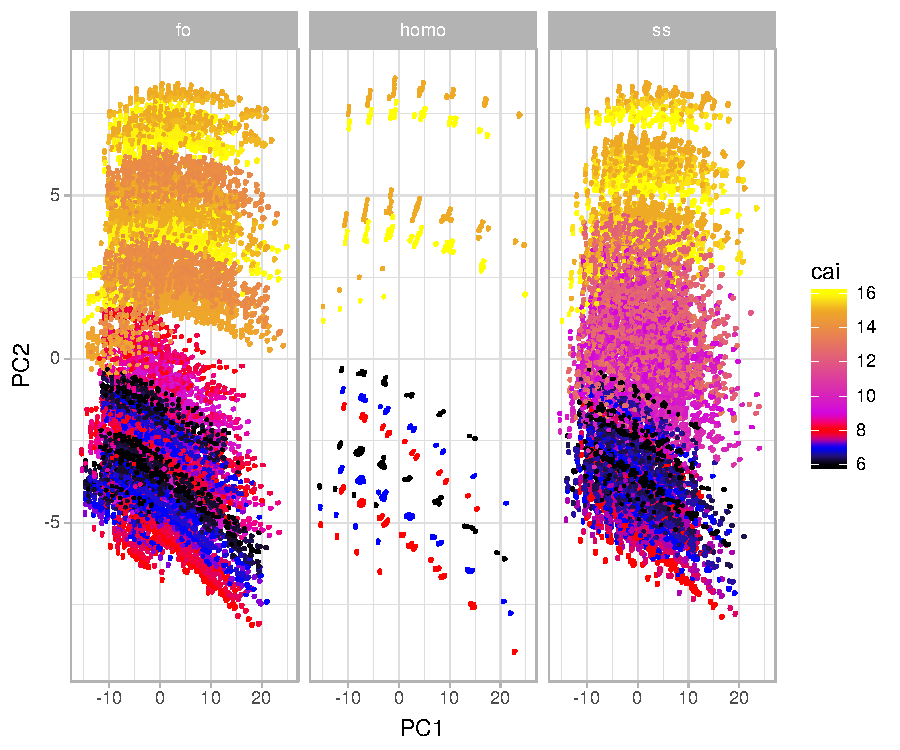
\includegraphics[width=0.65\linewidth]{img/pca.pdf}
\caption{asd} 
\end{figure}
\end{frame}

\begin{frame}
	\frametitle{Footprint and Entropy calculation}
	We use five properties to characterize the ligand field and generate a five dimensional distribution:
	\begin{itemize}
	\item total charge
	\item total valence electrons
	\item electronegativity of the connecting atom
	\item $^{\textrm{lc}}_{\textrm{ax,eq}}\chi_1 = \sum{EN_{\textrm{CA}} \cdot EN_i}$
	\item $^{\textrm{lc}}_{\textrm{ax,eq}}\chi^\prime_1 = \sum{EN_{\textrm{CA}} - EN_i}$
	
	\end{itemize}
	We then calculate the entropy, $H_{\textrm{KDE}}$, of the Kernel Density Estimated distrbution.
\end{frame}

\begin{frame}
\frametitle{Correlation analysis for strongly symmetric monodentates }
\begin{figure}
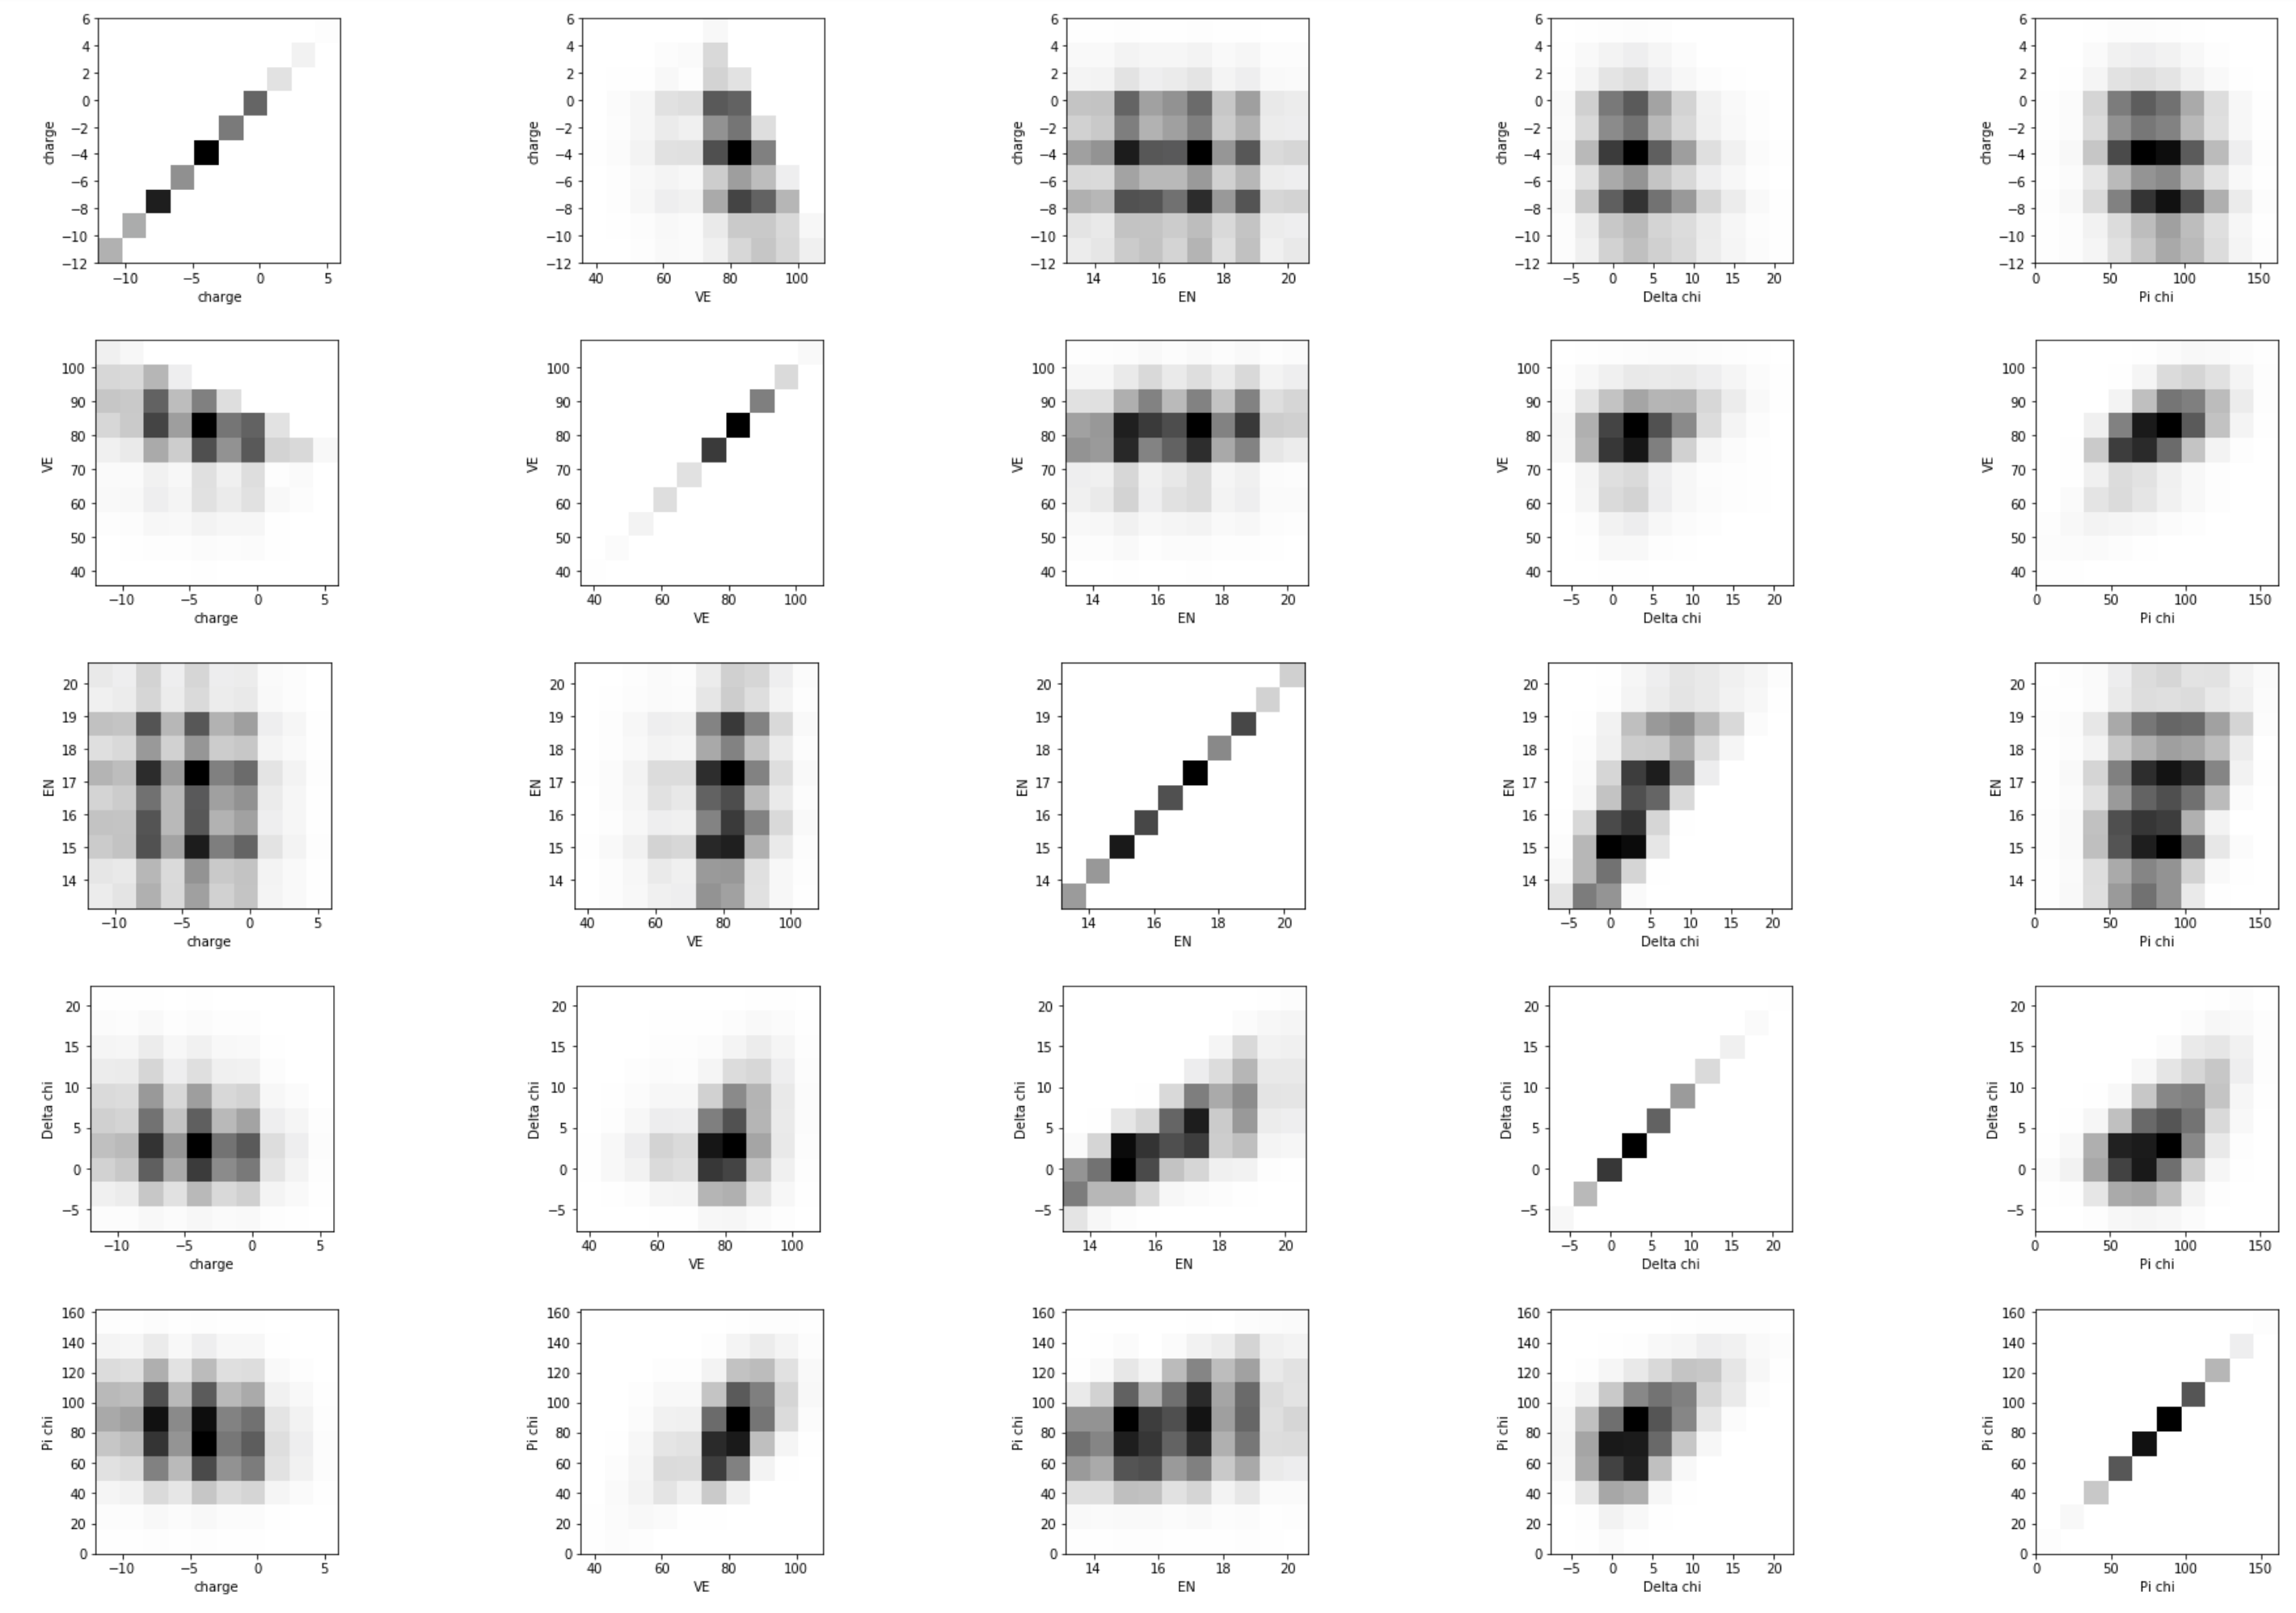
\includegraphics[width=0.65\linewidth]{img/strongsymMonodentates_PairwiseCorr.png}
\end{figure}
\end{frame}

\begin{frame}
\frametitle{Example of KDE slice}
Dimensions $^{\textrm{lc}}_{\textrm{ax,eq}}\chi_1$ vs. charge in $H_{\textrm{KDE}}$ for strongly symmetric monodentates.
\begin{figure}[ht] 
	\begin{minipage}[b]{0.5\linewidth}
		\centering
		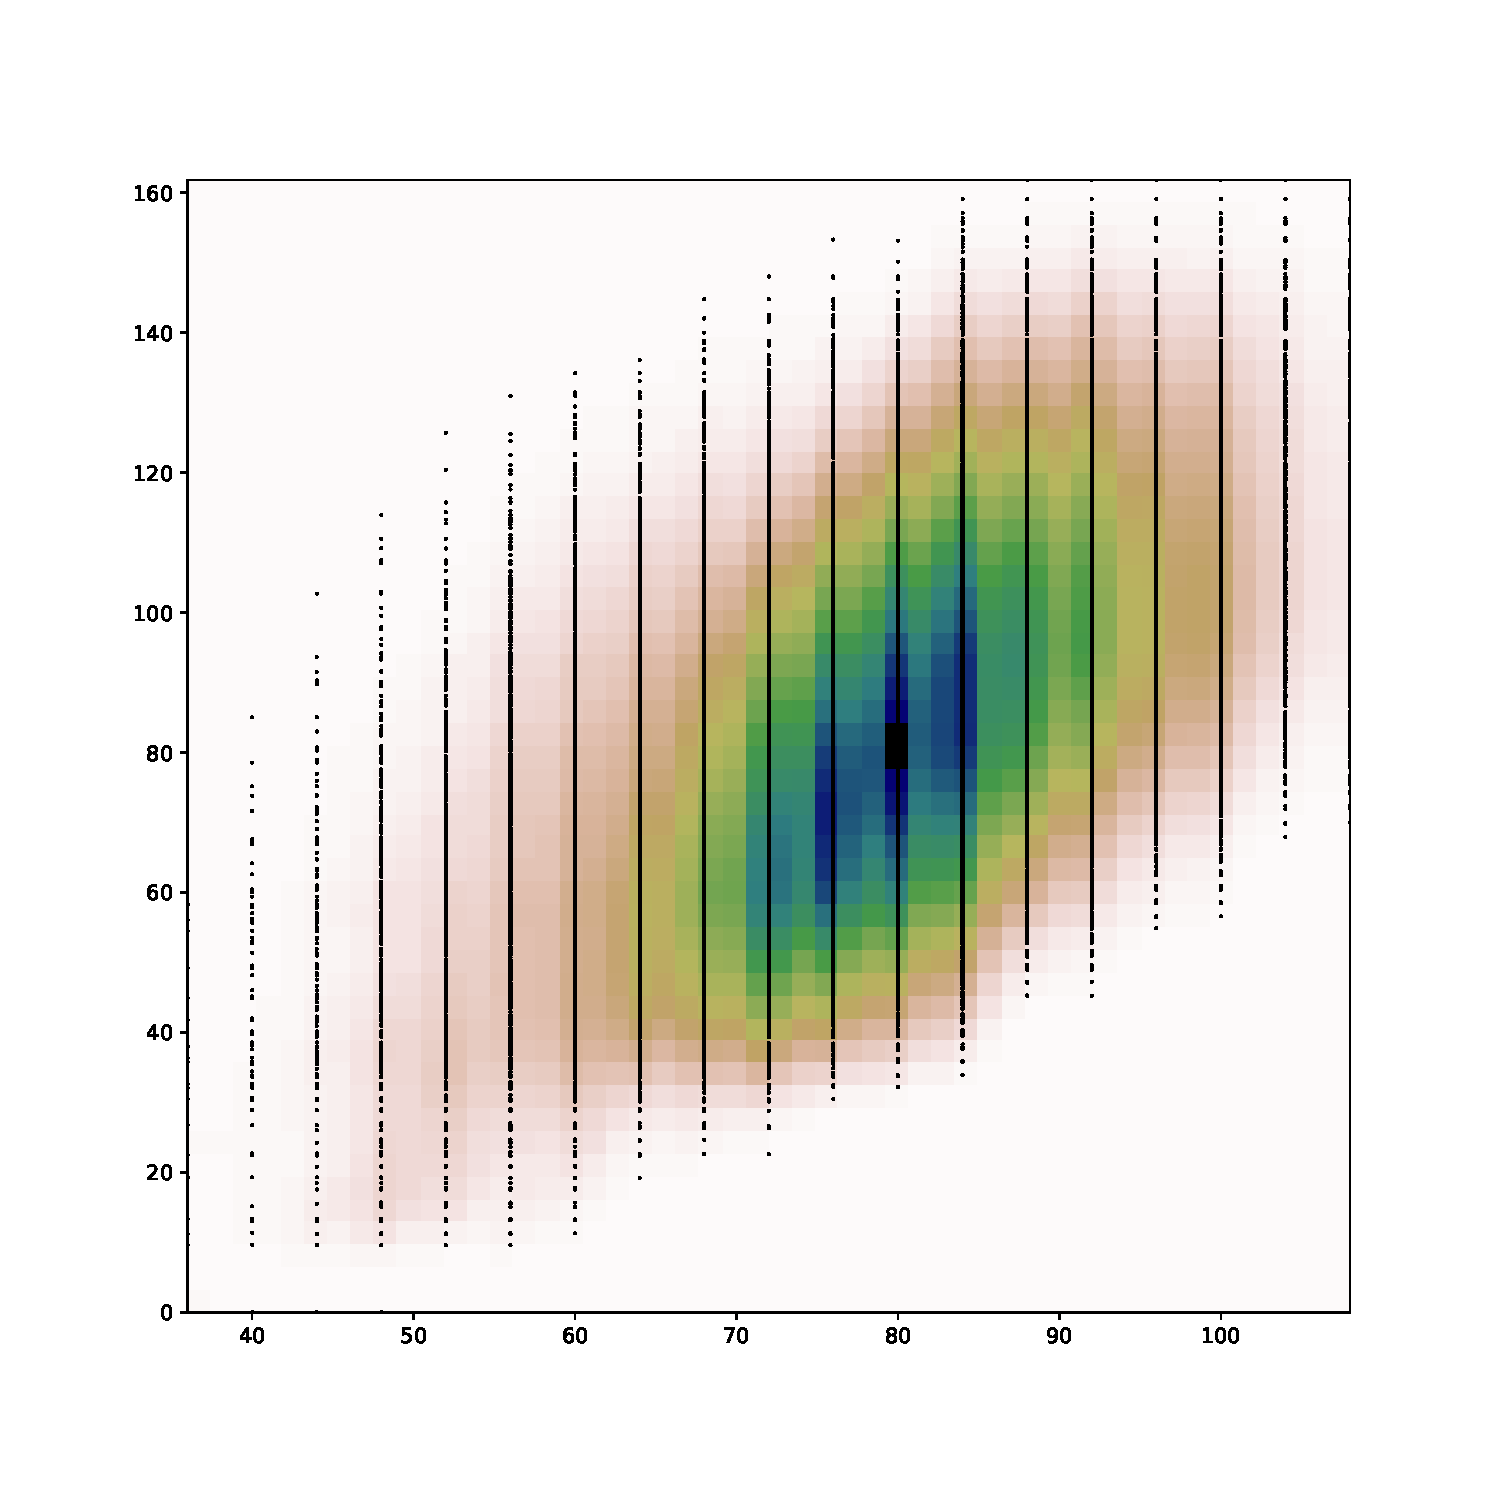
\includegraphics[width=1\linewidth]{img/strongsymMonodentates_heatmap.pdf} 
		\vspace{2ex}
	\end{minipage}%%
	\begin{minipage}[b]{0.5\linewidth}
		\centering
		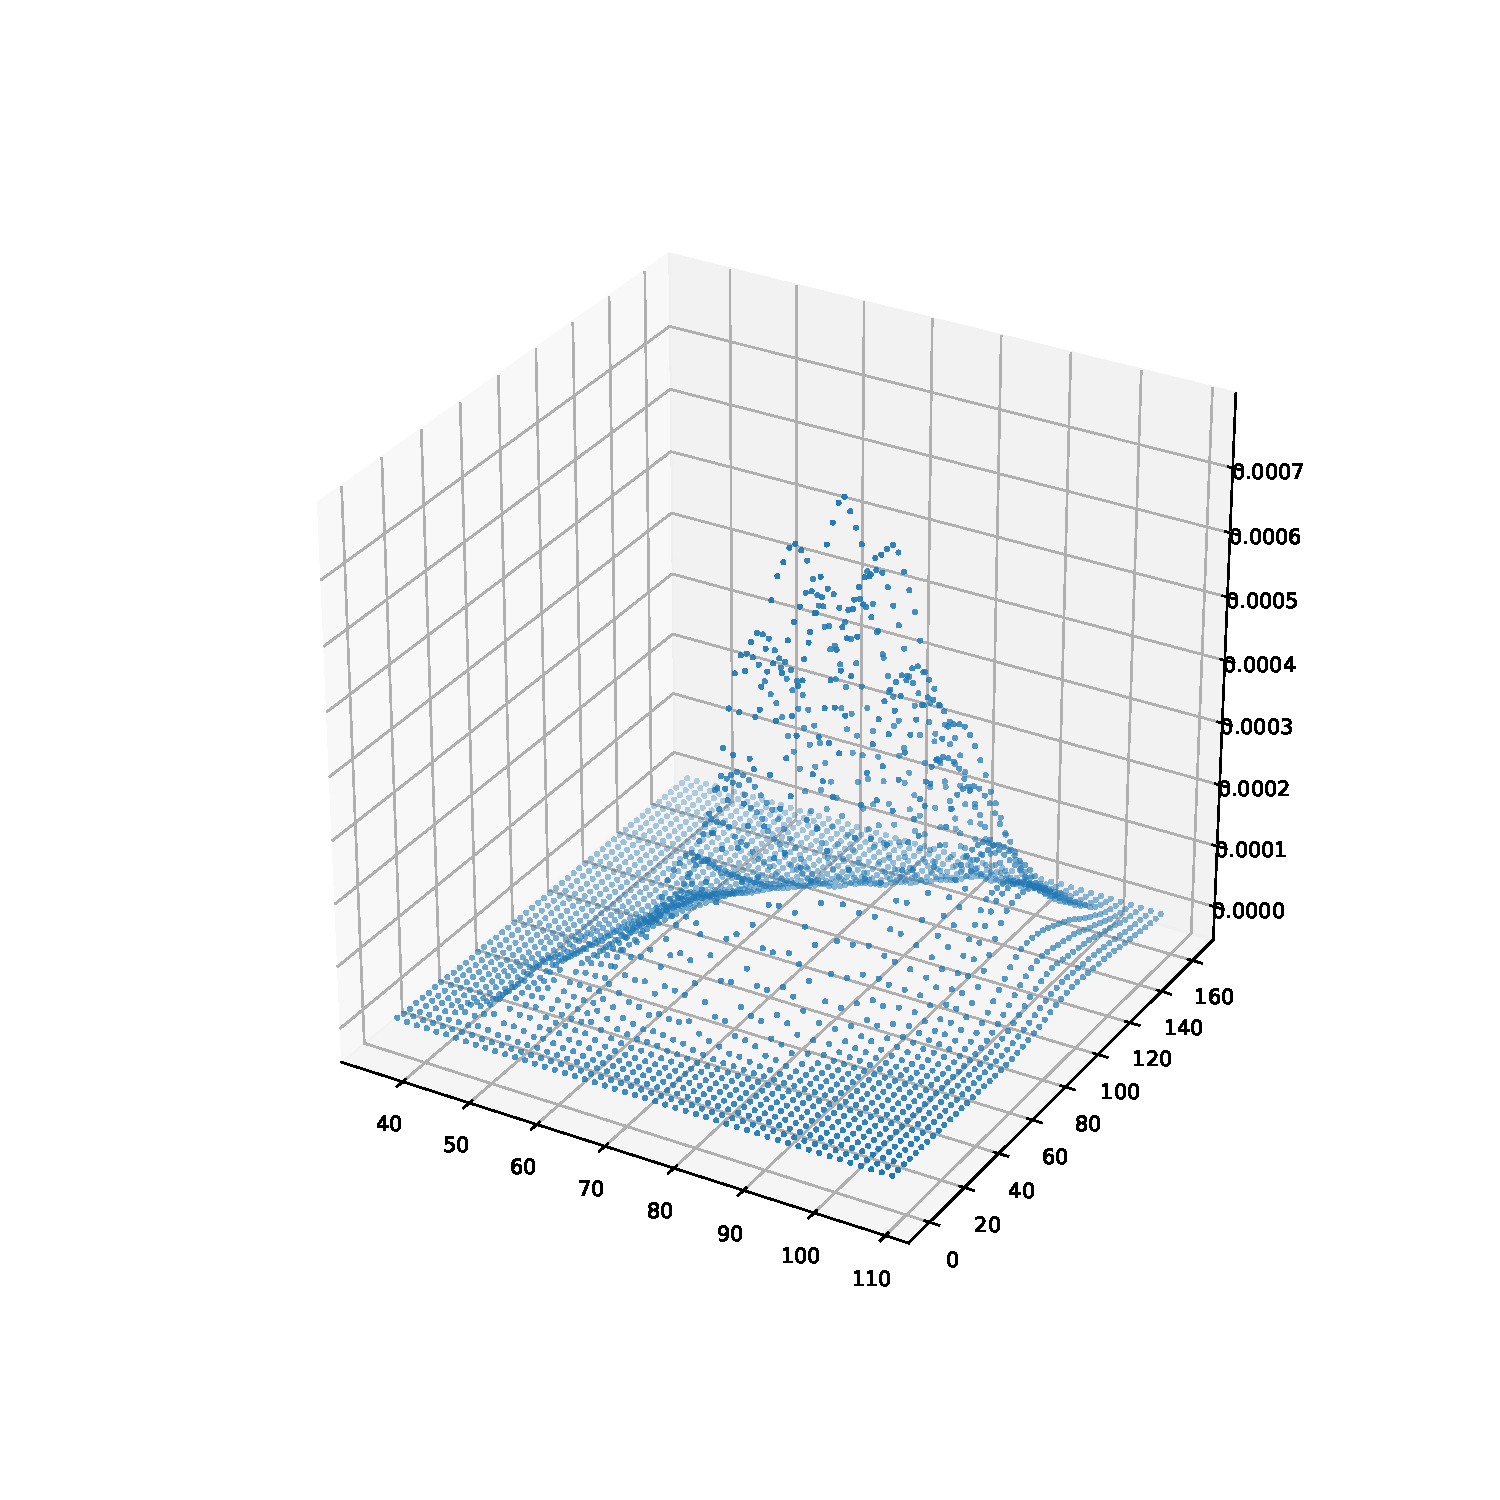
\includegraphics[width=1\linewidth]{img/strongsymMonodentates_3Dhists.pdf} 
		\vspace{2ex}
	\end{minipage} 
\end{figure}
\end{frame}

\begin{frame}
\frametitle{Monodentate Footprints}
	\begin{table}[]
	\centering
	\caption{Entropic footprint}
	\label{tab:ent-footprint}
	\begin{tabular}{lcr}
		\toprule
		Set 					    &  $H_{\textrm{KDE}}^{\textrm{monodent}}$   & $H_{\textrm{KDE}}^{\textrm{bident}}$ \\
		\midrule
		Homoleptics                 &  19.7  & 15.63   \\[0.1cm]
		"5+1" symmetric             &  13.7  & -       \\[0.1cm]
		Strongly symmetric AC       &  -     & 9.47    \\[0.1cm]
		Strongly symmetric ADC      &  12.70 & 5.53    \\[0.1cm]
		"4+2" symmetric             &  12.70 & 9.47    \\[0.1cm] 
		Weakly symmetric            &  8.1   &         \\[0.1cm]
		Equatorially asymmetric AC  &  -     & 10.04   \\[0.1cm]
		Equatorially asymmetric ADC &        &         \\[0.1cm]

		\bottomrule
	\end{tabular}
	\end{table}
\end{frame}

\begin{frame}
\frametitle{Entropy histogram}
\begin{figure}
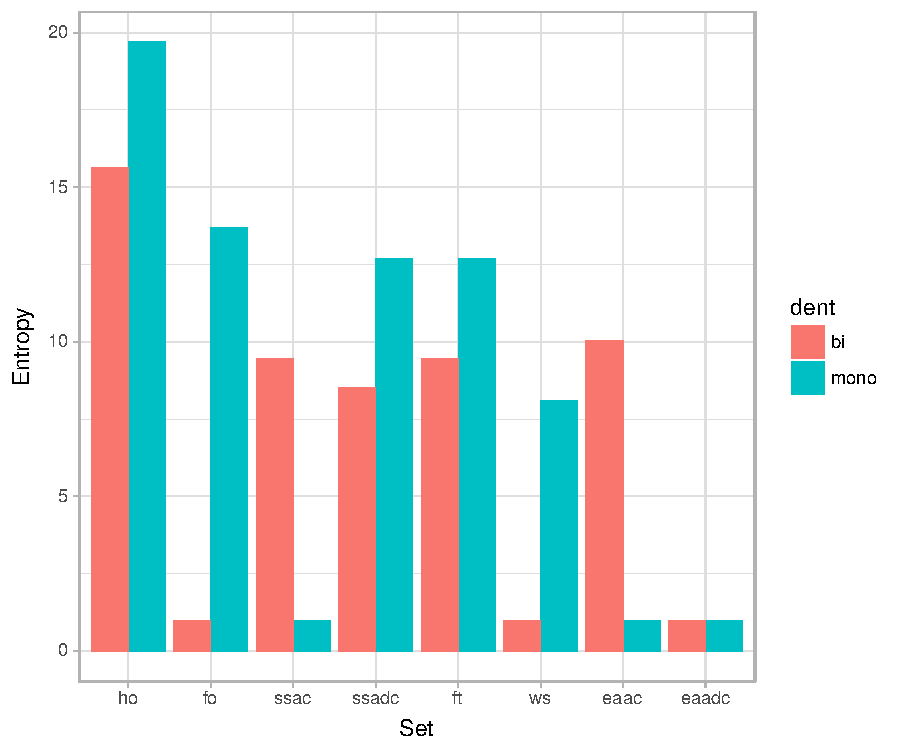
\includegraphics[width=0.7\linewidth]{img/ent.pdf}
\end{figure}
\end{frame}

%
%\begin{frame}
%\frametitle{Actual calculations}
%The calculations, colored by convergence fitness.
%\begin{figure}
%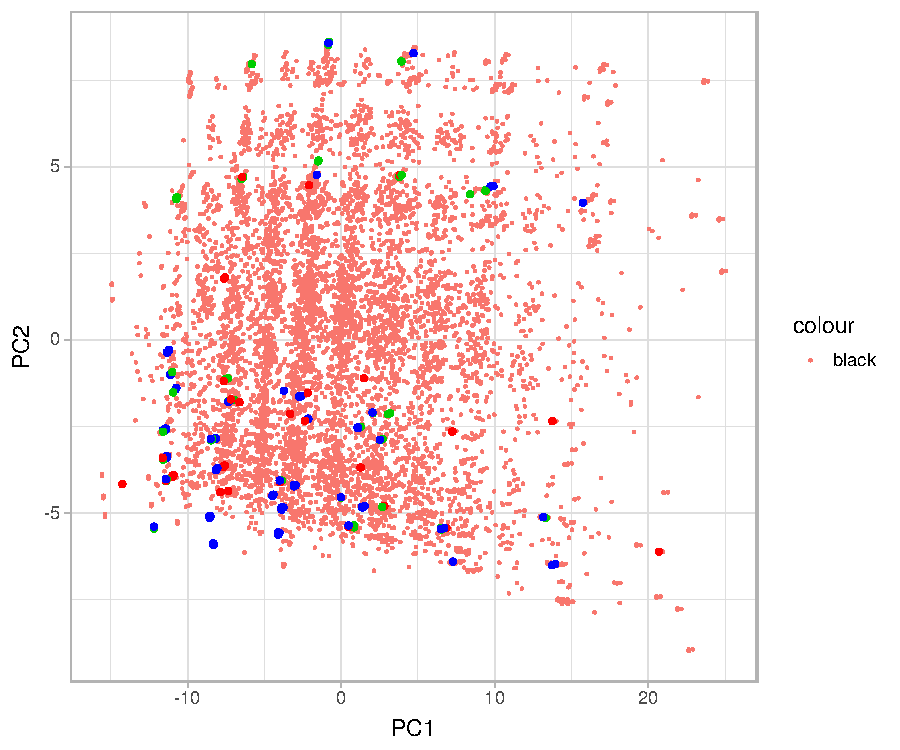
\includegraphics[width=0.7\linewidth]{img/pcaWithCalcs.pdf}
%\end{figure}
%\end{frame}

\begin{frame}
\frametitle{Mono-Heavy-Atomic Isoelectronic Ligand Distribution}
\begin{figure}[ht] 
	\label{ fig7} 
	\begin{minipage}[b]{0.5\linewidth}
		\centering
		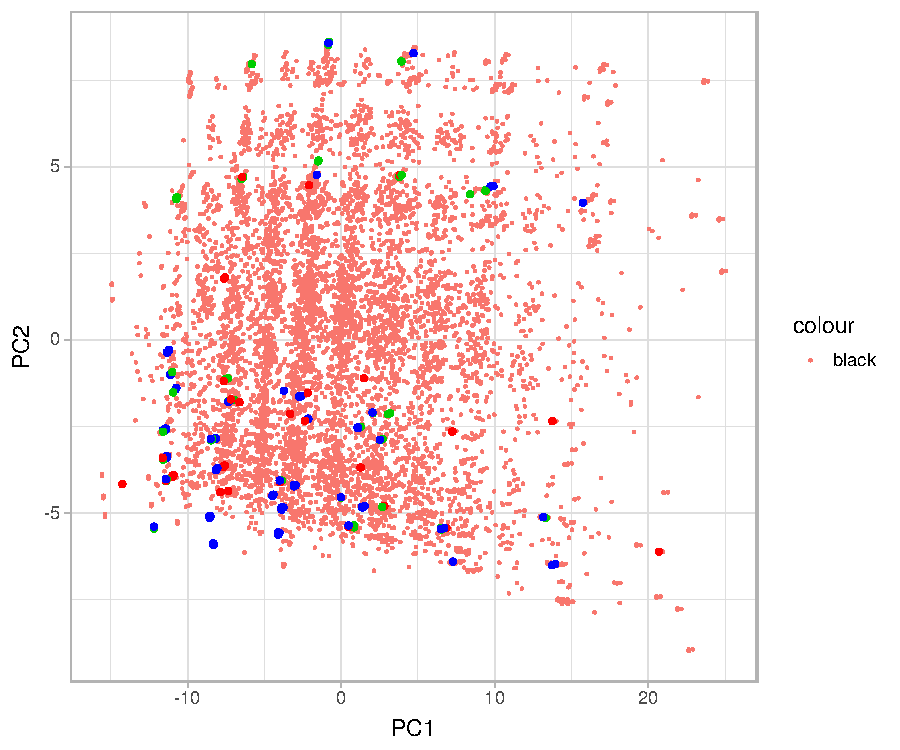
\includegraphics[width=.6\linewidth]{img/pcaWithCalcs.pdf} 
%		\vspace{8ex}
	\end{minipage}%%
	\begin{minipage}[b]{0.5\linewidth}
		\centering
		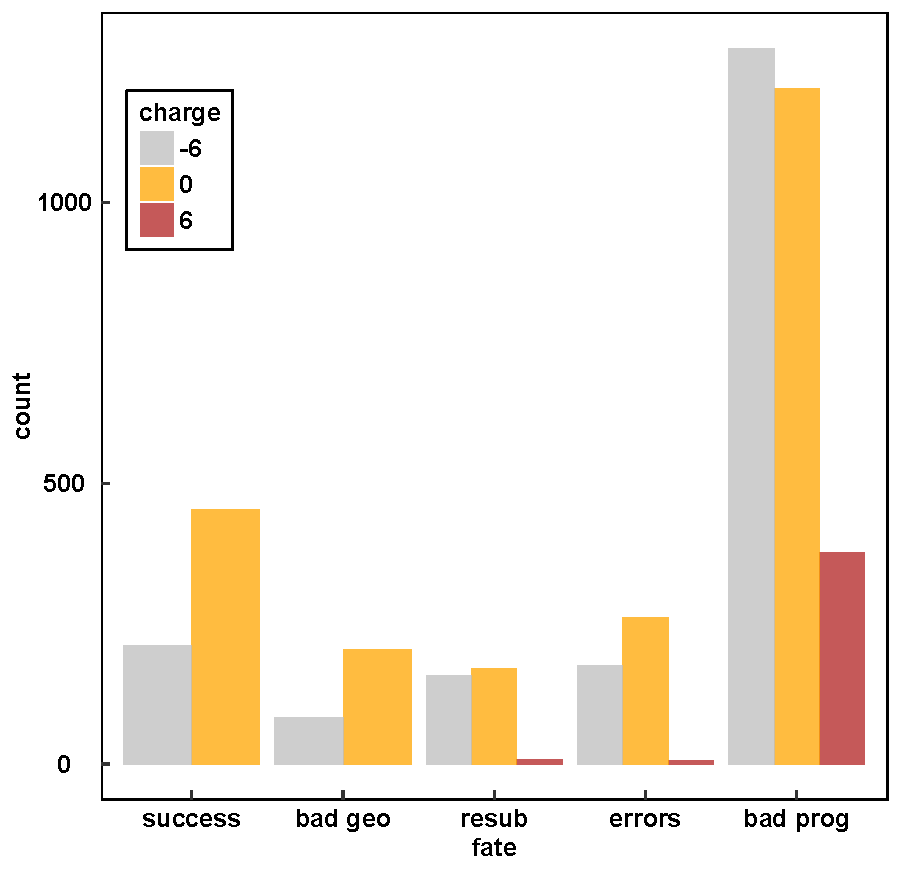
\includegraphics[width=.6\linewidth]{img/fateByCharge.pdf} 
%		\vspace{8ex}
	\end{minipage} 
	\begin{minipage}[b]{0.5\linewidth}
		\centering
		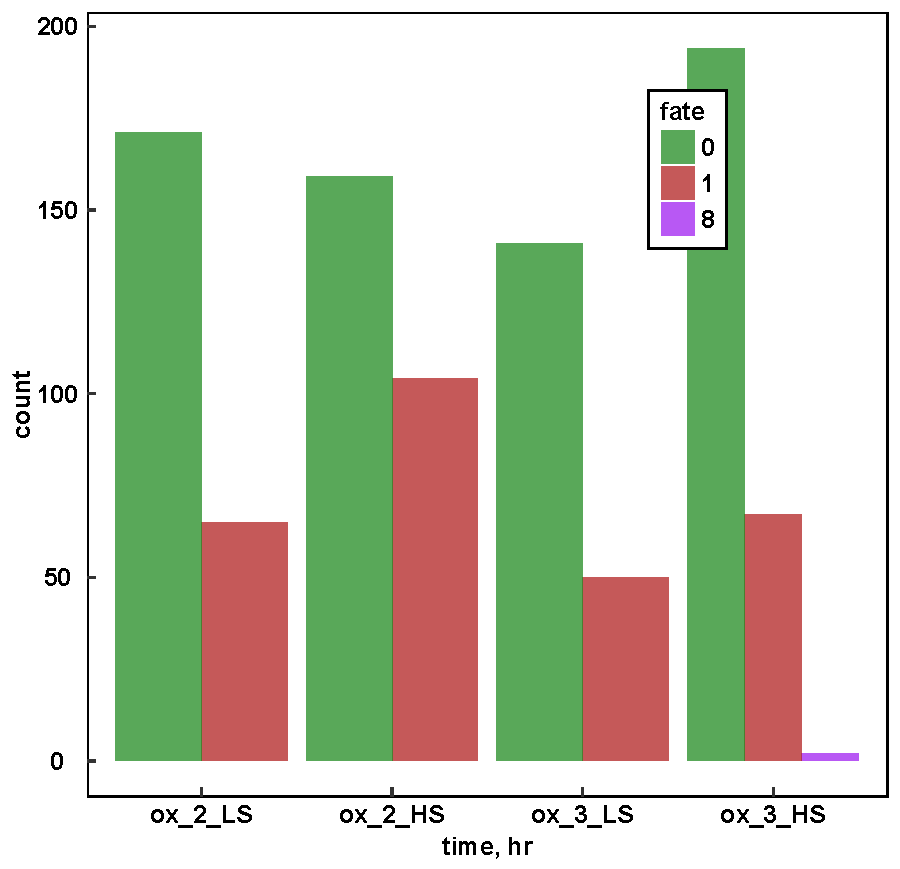
\includegraphics[width=.6\linewidth]{img/fateBytype.pdf} 
%		\vspace{4ex}
	\end{minipage}%% 
	\begin{minipage}[b]{0.5\linewidth}
		\centering
		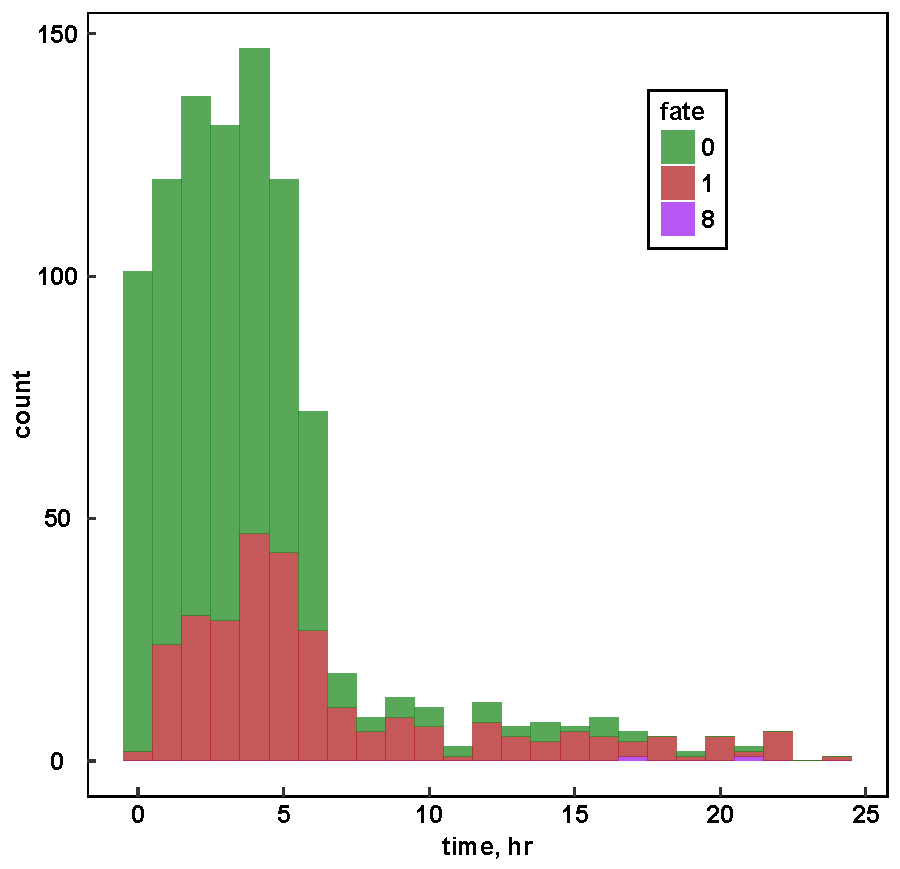
\includegraphics[width=.6\linewidth]{img/timeByfate.pdf} 
%		\vspace{4ex}
	\end{minipage} 
\end{figure}
\end{frame}


\begin{frame}
\begin{itemize}
\item 0: [NH3], [N]\#[N], [C+]\#[O-], [C+]\#[NH-]
\item 1: [CH+]=[CH3-]
\item 8: [OH2-]-[PH+], [P+]=[OH-], [PH+]-[OH2-], [NH2-]=[CH+]

\end{itemize}
\end{frame}


% % % % % % % % % % % % % % % %
%backup of the setsizes and entropies for individual mono/bi split sets
% % % % % % % % % % % % % % % %
%\begin{frame}
%\frametitle{Monodentate Sets}
%The sizes of the subsets of the monodentate octahedral space.
%\begin{table}[]
%	\centering
%%	\caption{The sizes of the subsets of the monodentate octahedral space.}
%	\label{tab:space-sizes-mono}
%	\begin{tabular}{llcr}
%		\toprule
%		Set 					& description		       & formula					        	   & size \\
%		\midrule
%		Homoleptics             & eq = ax                  & $\frac{405!}{404! \cdot  1!}$           & 405        \\[0.1cm]
%		"5+1" symmetric         & eq = ax1 $\neq$ ax2      & $\frac{405!}{403! \cdot  1! \cdot  1!}$ & 163,620    \\[0.1cm]
%		Strongly symmetric      & eq $\neq$ ax             & $\frac{405!}{403! \cdot  1! \cdot  1!}$ & 163,620    \\[0.1cm]
%		"4+2" symmetric         & eq1 $\neq$ eq2 = ax      & $\frac{405!}{403! \cdot  1! \cdot 1!}$  & 163,620    \\[0.1cm]
%		Equatorially asymmetric & eq1 $\neq$ eq2 $\neq$ ax & $\frac{405!}{402! \cdot  3!}$           & 10,989,810 \\[0.1cm]
%		Weakly symmetric        & eq $\neq$ ax1 $\neq$ ax2 & $\frac{405!}{402! \cdot  2! \cdot  1!}$ & 32,969,430 \\[0.1cm]
%		Complete Heteroleptics  & $L_i \neq L_j$           & $\frac{405!}{399! \cdot  6!}$           & $\approx 5.9 \cdot 10^{12}$ \\[0.1cm]
%		Octahedral Space        & all                      & $405^6                      $           & $\approx 4.4 \cdot 10^{15}$ \\
%		\bottomrule
%	\end{tabular}
%	\end{table}
%\end{frame}
%
%\begin{frame}
%	\frametitle{Bidentate Sets}
%	The sizes of the subsets of the bidentate octahedral space.
%	
%	\begin{table}[]
%	\centering
%%	\caption{The sizes of the subsets of the bidentate octahedral space.}
%	\label{tab:space-sizes-bi}
%	\begin{tabular}{llcr}
%		\toprule
%		Set 					& description		       & formula					        	 & size \\
%		\midrule
%		Homoleptics             & eq = ax                  & $\frac{148!}{147! \cdot  1!}$           & 148        \\[0.1cm]
%		Strongly symmetric AC   & eq $\neq$ ax             & $\frac{148!}{146! \cdot  1! \cdot  1!}$ & 21,756    \\[0.1cm]
%		Strongly symmetric ADC  & eq $\neq$ ax             & $405 \cdot  148$                        & 59,940    \\[0.1cm]
%		"4+2" symmetric         & eq1 $\neq$ eq2 = ax      & $\frac{148!}{146! \cdot  1! \cdot 1!}$  & 21,756    \\[0.1cm]
%		Equatorially asymmetric AC & eq1 $\neq$ eq2 $\neq$ ax & $\frac{148!}{145! \cdot  3!}$        & 529,396 \\[0.1cm]
%		Equatorially asymmetric ADC& eq1 $\neq$ eq2 $\neq$ ax & $\frac{405 \cdot 148!}{146! \cdot  2!}$& 4,405,590 \\[0.1cm]
%		Weakly symmetric        & eq $\neq$ ax1 $\neq$ ax2 & $\frac{405! \cdot 148}{403! \cdot  2!}$ & 12,107,880 \\[0.1cm]
%		\bottomrule
%	\end{tabular}
%	\end{table}
%\end{frame}
%
%\begin{frame}
%\frametitle{Monodentate Footprints}
%	\begin{table}[]
%	\centering
%	\caption{Entropic footprint}
%	\label{tab:ent-footprint}
%	\begin{tabular}{lcr}
%		\toprule
%		Set 					    &  $H_{\textrm{KDE}}^{\textrm{monodent}}$   & $H_{\textrm{KDE}}^{\textrm{bident}}]$ \\
%		\midrule
%		Homoleptics                 &  19.7  & 15.63   \\[0.1cm]
%		"5+1" symmetric             &  13.7  & -       \\[0.1cm]
%		Strongly symmetric AC       &  -     & 9.47    \\[0.1cm]
%		Strongly symmetric ADC      &  12.70 & 5.53    \\[0.1cm]
%		"4+2" symmetric             &  12.70 & 9.47    \\[0.1cm] 
%		Weakly symmetric            &  8.1   &         \\[0.1cm]
%		Equatorially asymmetric AC  &  -     & 10.04   \\[0.1cm]
%		Equatorially asymmetric ADC &        &         \\[0.1cm]
%
%		\bottomrule
%	\end{tabular}
%	\end{table}
%\end{frame}


\end{document}